\documentclass{extbook}[14pt]
\usepackage{multicol, enumerate, enumitem, hyperref, color, soul, setspace, parskip, fancyhdr, amssymb, amsthm, amsmath, bbm, latexsym, units, mathtools}
\everymath{\displaystyle}
\usepackage[headsep=0.5cm,headheight=0cm, left=1 in,right= 1 in,top= 1 in,bottom= 1 in]{geometry}
\usepackage{dashrule}  % Package to use the command below to create lines between items
\newcommand{\litem}[1]{\item #1

\rule{\textwidth}{0.4pt}}
\pagestyle{fancy}
\lhead{}
\chead{Answer Key for Progress Quiz 10 Version B}
\rhead{}
\lfoot{6232-9639}
\cfoot{}
\rfoot{Fall 2020}
\begin{document}
\textbf{This key should allow you to understand why you choose the option you did (beyond just getting a question right or wrong). \href{https://xronos.clas.ufl.edu/mac1105spring2020/courseDescriptionAndMisc/Exams/LearningFromResults}{More instructions on how to use this key can be found here}.}

\textbf{If you have a suggestion to make the keys better, \href{https://forms.gle/CZkbZmPbC9XALEE88}{please fill out the short survey here}.}

\textit{Note: This key is auto-generated and may contain issues and/or errors. The keys are reviewed after each exam to ensure grading is done accurately. If there are issues (like duplicate options), they are noted in the offline gradebook. The keys are a work-in-progress to give students as many resources to improve as possible.}

\rule{\textwidth}{0.4pt}

\begin{enumerate}\litem{
Determine the appropriate model for the graph of points below.

\begin{center}
    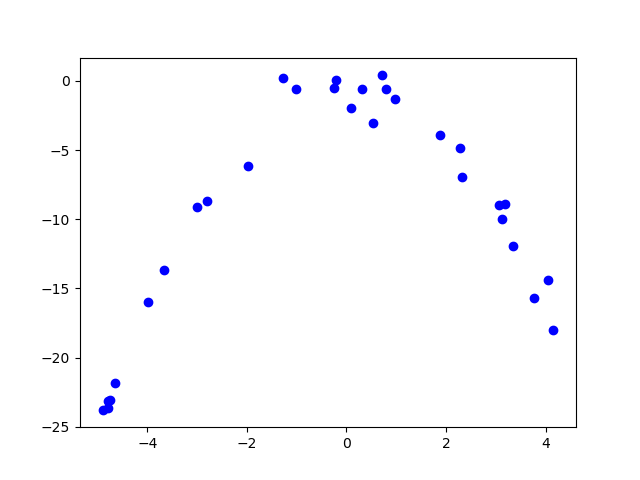
\includegraphics[width=0.5\textwidth]{../Figures/identifyModelGraph12B.png}
\end{center}




The solution is \( \text{Non-linear Power model} \), which is option A.\begin{enumerate}[label=\Alph*.]
\item \( \text{Non-linear Power model} \)

For this to be the correct option, we need to see a polynomial or rational shape.
\item \( \text{Exponential model} \)

For this to be the correct option, we want an extremely slow change early, then a rapid change later.
\item \( \text{Linear model} \)

For this to be the correct option, we need to see a mostly straight line of points.
\item \( \text{Logarithmic model} \)

For this to be the correct option, we want a rapid change early, then an extremely slow change later.
\item \( \text{None of the above} \)

For this to be the correct option, we want to see no pattern in the points.
\end{enumerate}

\textbf{General Comment:} This question is testing if you can associate the models with their graphical representation. If you are having trouble, go back to the corresponding Core module to learn about the specific function you are having trouble recognizing.
}
\litem{
Solve the modeling problem below, if possible.

\begin{center}
    \textit{ In CHM2045L, Brittany created a 21 liter 23 percent solution of chemical $\chi$ using two different solution percentages of chemical $\chi$. When she went to write her lab report, she realized she forgot to write the amount of each solution she used! If she remembers she used 18 percent and 44 percent solutions, what was the amount she used of the 44 percent solution? }
\end{center}


The solution is \( 4.04 \), which is option B.\begin{enumerate}[label=\Alph*.]
\item \( 16.96 \)

This is the concentration of 18 percent solution.
\item \( 4.04 \)

*This is the correct option.
\item \( 10.50 \)

This would be correct if Brittany used equal parts of each solution.
\item \( 15.32 \)

This was a random value. If this was not a guess, contact the coordinator to talk about how you got this value.
\item \( \text{There is not enough information to solve the problem.} \)

You may have chose this if you thought you needed to know how much of the second solution was used in the problem. Remember that the total minus the first solution would give you the second amount used.
\end{enumerate}

\textbf{General Comment:} Build the model exactly as you did in Module 9M. Then, solve for the volume you are looking for.
}
\litem{
Determine the appropriate model for the graph of points below.

\begin{center}
    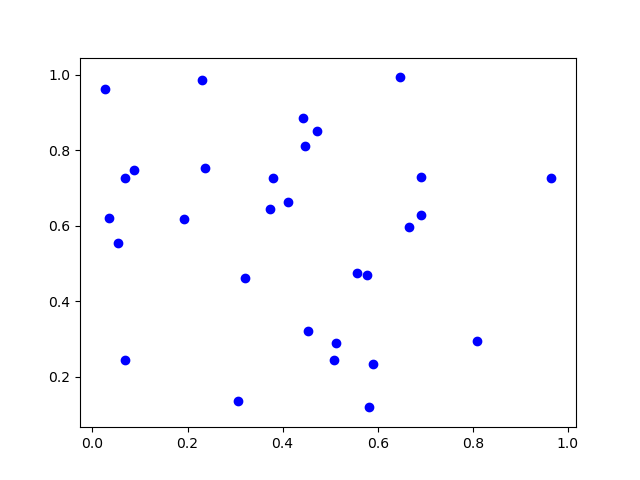
\includegraphics[width=0.5\textwidth]{../Figures/identifyModelGraph12CopyB.png}
\end{center}




The solution is \( \text{None of the above} \), which is option E.\begin{enumerate}[label=\Alph*.]
\item \( \text{Non-linear Power model} \)

For this to be the correct option, we need to see a polynomial or rational shape.
\item \( \text{Exponential model} \)

For this to be the correct option, we want an extremely slow change early, then a rapid change later.
\item \( \text{Linear model} \)

For this to be the correct option, we need to see a mostly straight line of points.
\item \( \text{Logarithmic model} \)

For this to be the correct option, we want a rapid change early, then an extremely slow change later.
\item \( \text{None of the above} \)

For this to be the correct option, we want to see no pattern in the points.
\end{enumerate}

\textbf{General Comment:} This question is testing if you can associate the models with their graphical representation. If you are having trouble, go back to the corresponding Core module to learn about the specific function you are having trouble recognizing.
}
\litem{
Solve the modeling problem below, if possible.

\begin{center}
    \textit{ A new virus is spreading throughout the world. There were initially 8 many cases reported, but the number of confirmed cases has doubled every 4 days. How long will it be until there are at least 100000 confirmed cases? }
\end{center}


The solution is \( \text{About } 55 \text{ days} \), which is option A.\begin{enumerate}[label=\Alph*.]
\item \( \text{About } 55 \text{ days} \)

* This is the correct option.
\item \( \text{About } 17 \text{ days} \)

You modeled the situation correctly but did not apply the properties of log correctly.
\item \( \text{About } 38 \text{ days} \)

You modeled the situation with $e$ as the base, but solved correctly otherwise.
\item \( \text{About } 15 \text{ days} \)

You modeled the situation with $e$ as the base and did not apply the properties of log correctly.
\item \( \text{There is not enough information to solve the problem.} \)

If you chose this option, please contact the coordinator to discuss why you think this is the case.
\end{enumerate}

\textbf{General Comment:} Set up the model the same as in Module 11M. Then, plug in 100000 and solve for $d$ in your model.
}
\litem{
For the scenario below, use the model for the volume of a cylinder as $V = \pi r^2 h$.

\begin{center}
    \textit{ Pringles wants to add 46 \text{percent} more chips to their cylinder cans and minimize the design change of their cans. They've decided that the best way to minimize the design change is to increase the radius and height by the same percentage. What should this increase be? }
\end{center}


The solution is \( \text{About } 13 \text{ percent} \), which is option C.\begin{enumerate}[label=\Alph*.]
\item \( \text{About } 21 \text{ percent} \)

This corresponds to solving correctly but treating both radius and height as equal contributors to the volume.
\item \( \text{About } 23 \text{ percent} \)

This corresponds to treating both radius and height as equal contributors and not solving correctly.
\item \( \text{About } 13 \text{ percent} \)

* This is the correct option.
\item \( \text{About } 4 \text{ percent} \)

This corresponds to not solving for the increase properly.
\item \( \text{None of the above} \)

If you chose this, please contact the coordinator to discus how you solved the problem.
\end{enumerate}

\textbf{General Comment:} Remember that when plugging the increases of values in, you need to treat it as that percentage above 100. For example, a 5 percent increase means 105 percent.
}
\litem{
Using the scenario below, model the situation using an exponential function and a base of $\frac{1}{2}$. Then, solve for the half-life of the element, rounding to the nearest day.

\begin{center}
    \textit{ The half-life of an element is the amount of time it takes for the element to decay to half of its initial starting amount. There is initially 736 grams of element $X$ and after 11 years there is 184 grams remaining. }
\end{center}


The solution is \( \text{About } 1825 \text{ days} \), which is option B.\begin{enumerate}[label=\Alph*.]
\item \( \text{About } 730 \text{ days} \)

This models half-life as a linear function.
\item \( \text{About } 1825 \text{ days} \)

* This is the correct option.
\item \( \text{About } 2555 \text{ days} \)

This uses the correct model but a base of $e$ rather than $\frac{1}{2}$.
\item \( \text{About } 4380 \text{ days} \)

This uses the correct model but solves for the exponential constant incorrectly.
\item \( \text{None of the above} \)

Please contact the coordinator if you believe all the options above are incorrect.
\end{enumerate}

\textbf{General Comment:} The model should be $A(t) = A_0 (\frac{1}{2})^{kt}$, where $A(t)$ is the amount after $t$ years, $A_0$ is the initial amount, and $k$ is decay constant. To find the half-life, you need to solve for $k$ by using the amount after $x$ years, then solve for the time $t$ when $A = \frac{A_0}{2}$. Your answer would be in years, so convert to days.
}
\litem{
Solve the modeling problem below, if possible.

\begin{center}
    \textit{ In CHM2045L, Brittany created a 17 liter 24 percent solution of chemical $\chi$ using two different solution percentages of chemical $\chi$. When she went to write her lab report, she realized she forgot to write the amount of each solution she used! If she remembers she used 19 percent and 30 percent solutions, what was the amount she used of the 19 percent solution? }
\end{center}


The solution is \( 9.27 \), which is option A.\begin{enumerate}[label=\Alph*.]
\item \( 9.27 \)

*This is the correct option.
\item \( 7.73 \)

This is the concentration of 30 percent solution.
\item \( 7.18 \)

This was a random value. If this was not a guess, contact the coordinator to talk about how you got this value.
\item \( 8.50 \)

This would be correct if Brittany used equal parts of each solution.
\item \( \text{There is not enough information to solve the problem.} \)

You may have chose this if you thought you needed to know how much of the second solution was used in the problem. Remember that the total minus the first solution would give you the second amount used.
\end{enumerate}

\textbf{General Comment:} Build the model exactly as you did in Module 9M. Then, solve for the volume you are looking for.
}
\litem{
Solve the modeling problem below, if possible.

\begin{center}
    \textit{ A new virus is spreading throughout the world. There were initially 4 many cases reported, but the number of confirmed cases has doubled every 2 days. How long will it be until there are at least 100000 confirmed cases? }
\end{center}


The solution is \( \text{About } 30 \text{ days} \), which is option C.\begin{enumerate}[label=\Alph*.]
\item \( \text{About } 12 \text{ days} \)

You modeled the situation correctly but did not apply the properties of log correctly.
\item \( \text{About } 21 \text{ days} \)

You modeled the situation with $e$ as the base, but solved correctly otherwise.
\item \( \text{About } 30 \text{ days} \)

* This is the correct option.
\item \( \text{About } 10 \text{ days} \)

You modeled the situation with $e$ as the base and did not apply the properties of log correctly.
\item \( \text{There is not enough information to solve the problem.} \)

If you chose this option, please contact the coordinator to discuss why you think this is the case.
\end{enumerate}

\textbf{General Comment:} Set up the model the same as in Module 11M. Then, plug in 100000 and solve for $d$ in your model.
}
\litem{
For the information below, construct a linear model that describes the total time $T$ spent on the path in terms of the distance of a particular part of the path \textit{if we know that the time spent on each path was equal}.

\begin{center}
    \textit{ A bicyclist is training for a race on a hilly path. Their bike keeps track of their speed at any time, but not the distance traveled. Their speed traveling up a hill is 4 mph, 10 mph when traveling down a hill, and 6 mph when traveling along a flat portion. }
\end{center}


The solution is \( \text{The model can be found with the information provided, but isn't options 1-3.} \), which is option D.\begin{enumerate}[label=\Alph*.]
\item \( 20.000 D \)

The coefficient here is calculated as if you were trying to model the distance on the total path.
\item \( 0.517 D \)

This would be correct if we knew all parts of the path are equal length.
\item \( 240.000 D \)

The coefficient here is calculated by multiplying the distances together rather than adding.
\item \( \text{The model can be found with the information provided, but isn't options 1-3.} \)

* This is the correct option. Since the time spent on each path was equal, the distance of each path must be different. The model would be $0.250D_u + 0.100D_d + 0.167D_f$, where $D_u$ is distance traveling up the hill, $D_d$ is distance traveling down, and $D_f$ is distance traveling on a flat part.
\item \( \text{The model cannot be found with the information provided.} \)

If you chose this option, please contact the coordinator to discuss why you think we cannot model the situation.
\end{enumerate}

\textbf{General Comment:} Be sure you pay attention to the variable we are writing the model in terms of. To create the model with a single variable, we have to know that variable is the same throughout each path!
}
\litem{
For the scenario below, use the model for the volume of a cylinder as $V = \pi r^2 h$.

\begin{center}
    \textit{ Pringles wants to add 32 \text{percent} more chips to their cylinder cans and minimize the design change of their cans. They've decided that the best way to minimize the design change is to increase the radius and height by the same percentage. What should this increase be? }
\end{center}


The solution is \( \text{About } 10 \text{ percent} \), which is option C.\begin{enumerate}[label=\Alph*.]
\item \( \text{About } 11 \text{ percent} \)

This corresponds to not solving for the increase properly.
\item \( \text{About } 16 \text{ percent} \)

This corresponds to treating both radius and height as equal contributors and not solving correctly.
\item \( \text{About } 10 \text{ percent} \)

* This is the correct option.
\item \( \text{About } 15 \text{ percent} \)

This corresponds to solving correctly but treating both radius and height as equal contributors to the volume.
\item \( \text{None of the above} \)

If you chose this, please contact the coordinator to discus how you solved the problem.
\end{enumerate}

\textbf{General Comment:} Remember that when plugging the increases of values in, you need to treat it as that percentage above 100. For example, a 5 percent increase means 105 percent.
}
\end{enumerate}

\end{document}